%%%%%%%%%%%%%%%%%%%%%%%%%%%%%%%%%%%%%%%%%%%%%%%%%%%%%%%%%%%%%%%%%%%%%%%
%% 
%%%%%%%%%%%%%%%%%%%%%%%%%%%%%%%%%%%%%%%%%%%%%%%%%%%%%%%%%%%%%%%%%%%%%%%

\chapter{Hauptteil}
\label{sec:haupt}

Der Hauptteil kann aus den Kapiteln Aufgabenstellung, Konzept, Implementierung, Test, usw. je nach Arbeitsthema bestehen. innerhalb der \texttt{Abschlussarbeit.tex} wird der Grobaufbau der Arbeit definiert. Die Datei \texttt{header.tex} konfiguriert die Packages und alle Dokumenteigenschaften. Beide Dateien sollten bekannt sein und m�ssen bei Bedarf abge�ndert bzw. erweitert werden. Die eingebundenen Packages stellen neue M�glichkeiten bereit, einige sollen hier kurz vorgestellt werden.

\section{Abbildungen}
\label{sec:haupt:figure}

Das Einbinden von Grafiken soll an Abbildung \ref{fig:beispiel} gezeigt werden. Die Grafik selbst liegt entsprechend der Definition in der \texttt{header.tex} im Projekt-Unterordner "`Bilder"' und sollte zur guten Darstellung als png-Bilddatei oder als Vektorgrafik vorliegen.

\begin{figure}[htb]
\begin{center} 
  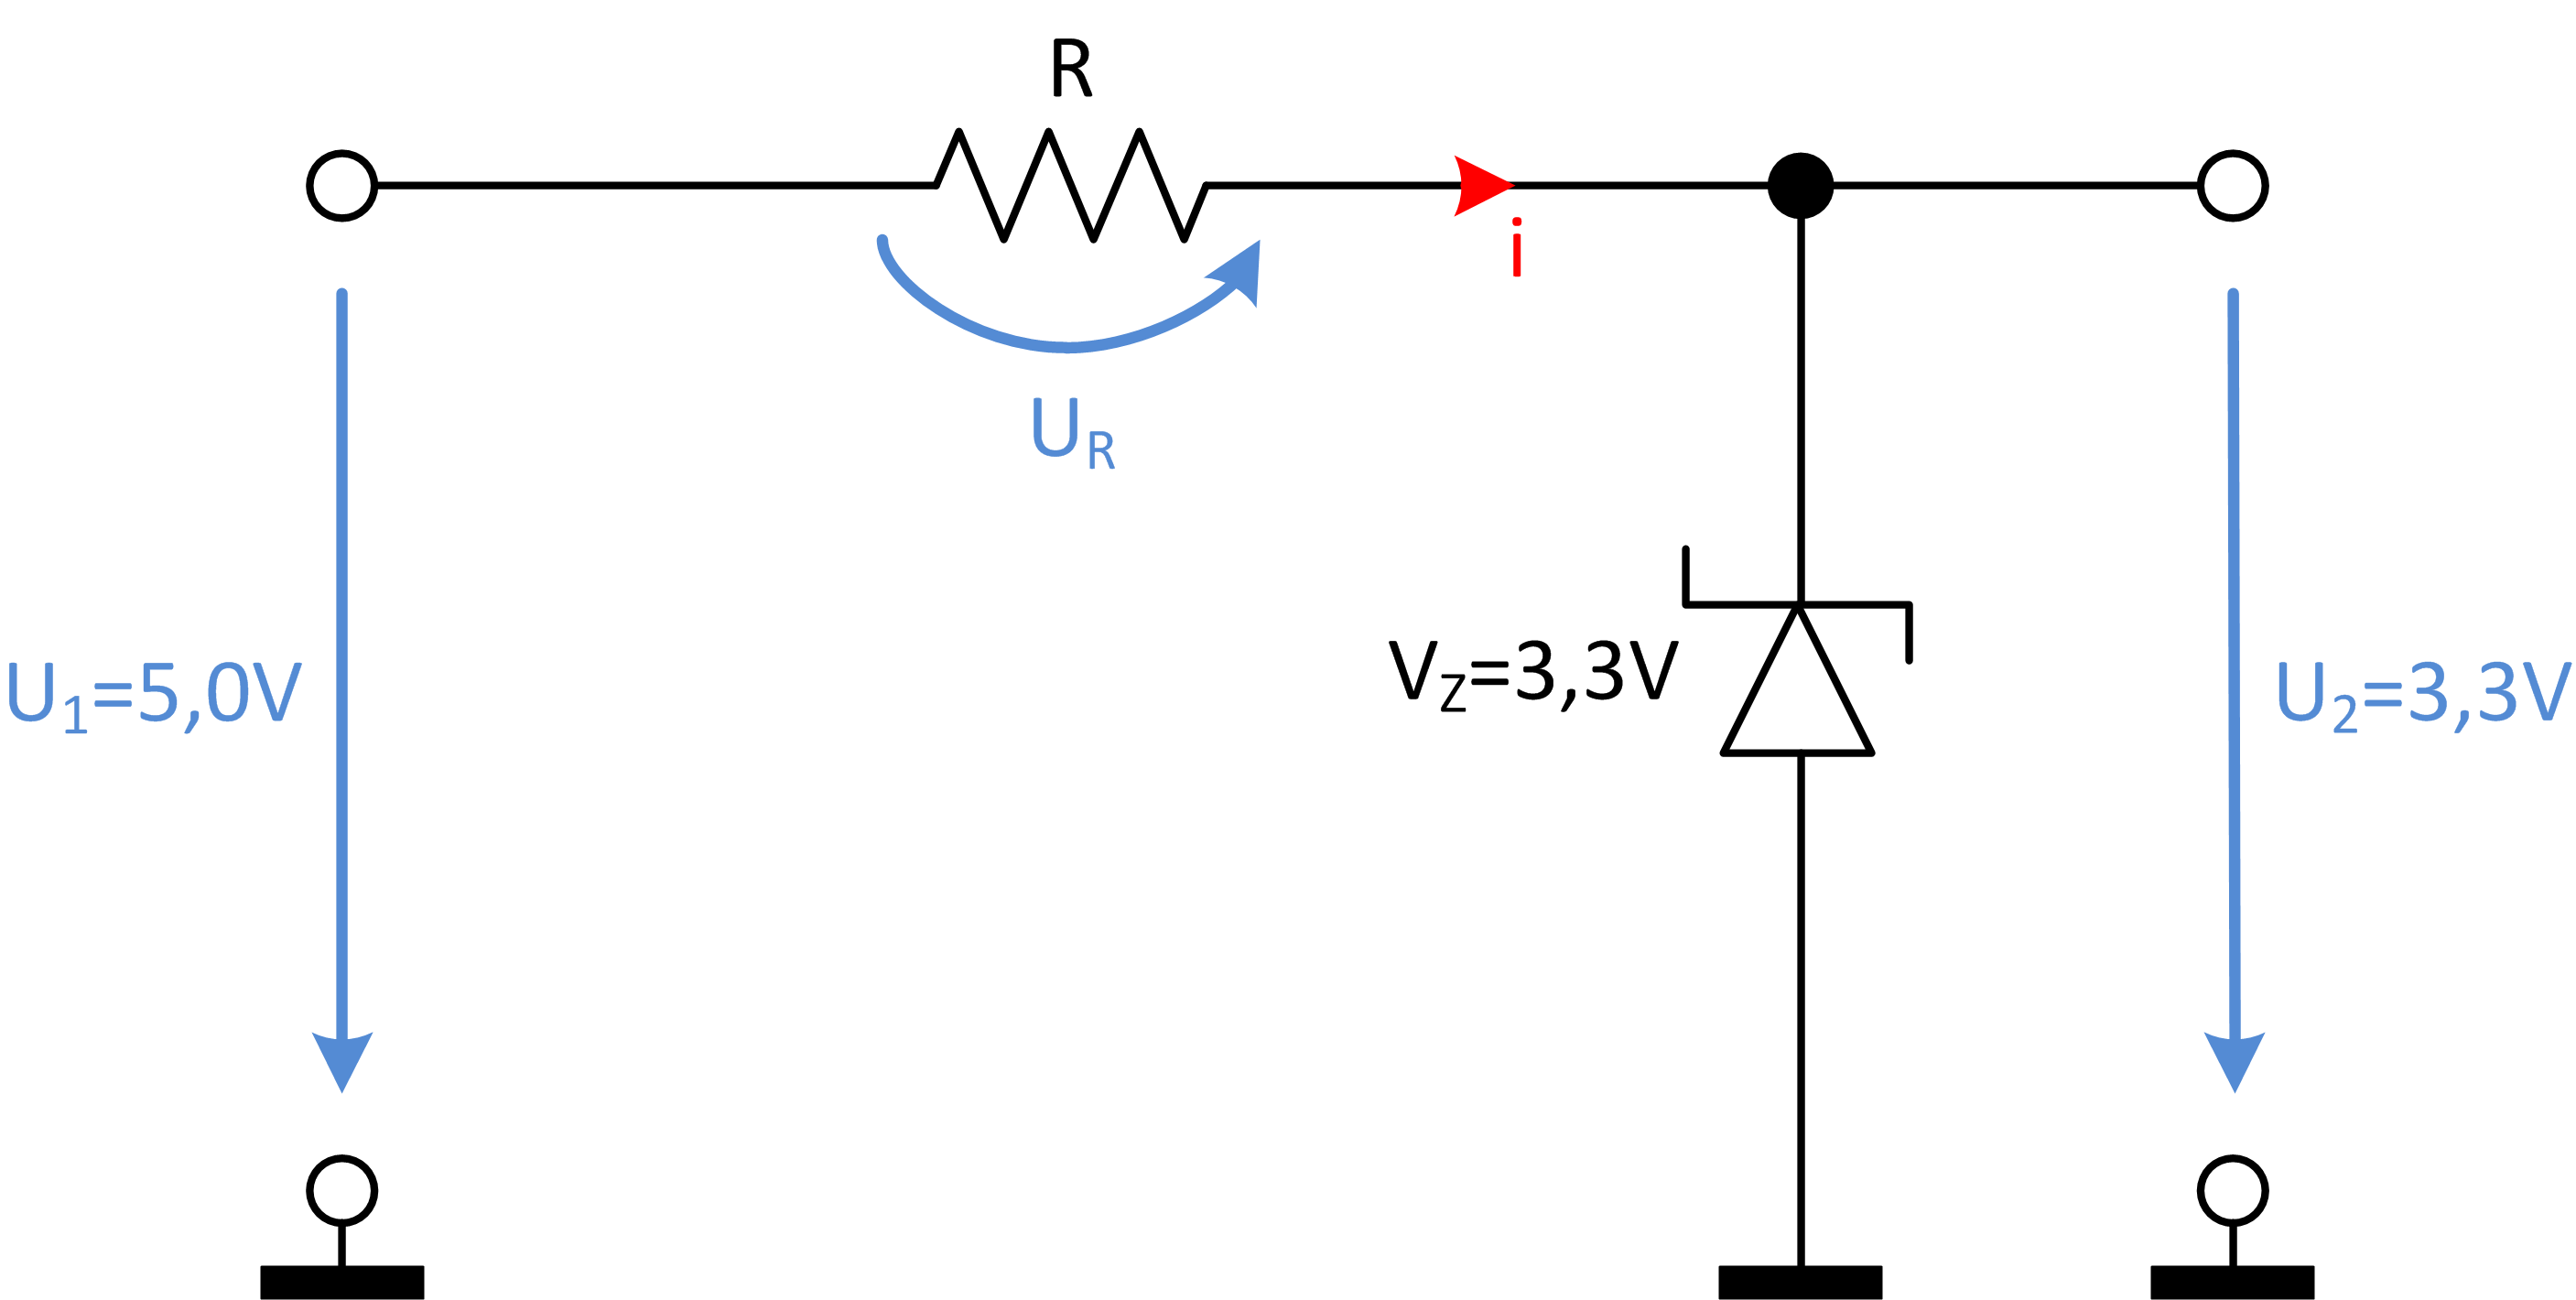
\includegraphics[width=0.60\textwidth]{Beispiel}  
  \caption{Ein Bild als Beispiel}
  \label{fig:beispiel}
\end{center}
\end{figure}
 
Die Positionsdefinition "`htb"' beschreibt die automatische Positionierung in LaTeX in der bevorzugten Reihenfolge "`here, top, buttom"'. Wenn man wei� was man tut und die Grafik in jedem Fall genau an der gew�hlten Stelle eingebunden werden soll ist "`h!"' zu nutzen. Ein Warning\todoedit{zu beachten}\ wird generiert wenn diese Anforderung nicht erf�llt werden kann\todoref{Zu dieser Aussage sollte noch eine Quelle angegeben werden}.
 
\section{Verschiedenes}
\label{sec:haupt:misc}

Ein Beispiel f�r eine nummerierte Tabelle mit Gro�buchstaben und einer speziellen Formatierung:
\begin{enumerate}[\bfseries (A) {-}]
  \item Das Kapitel \ref{sec:haupt} tr�gt den Titel \nameref{sec:haupt}\footnote{Die Nutzung von Nameref ist in vielen Situationen n�tzlich} und beginnt auf Seite \pageref{sec:haupt} 
  \item \SI{3}{\volt} liegt im Bereich zwischen \SIrange[range-units=single]{2,5}{3,5}{\volt}. Die Stromst�rke wird meist in der Einheit \si{\mA} angegeben und auch eine einfache Zahl wie bspw. \num{65536,128} l�sst sich mit dem Package \texttt{siunitx} sicher darstellen.
     
\end{enumerate}


\begin{lstlisting}[caption={\texttt{SCI.c} - SCI-Definitionen}, label=lst:scidefine]
	#define SCIBDH     SCI1BDH
	#define SCIBDL     SCI1BDL
	#define SCIC1      SCI1C1
	#define SCIC2      SCI1C2
	...                ...
\end{lstlisting}

\lstinputlisting[%
		caption=\texttt{wireless\_uart.c} - Auszug,%
		label=lst:scirx,%
		float=hbt,%
		frame={tbrl},%
		%firstline=1,%
		lastline=7,%
]{Sourcecode/bsp.c}

\begin{table}[htb]
\centering
	\begin{tabular}{llr}
	\toprule
	Device & Teiler & Baudrate [Baud]\\
	\midrule
	\multirow{2}{2.5cm}{Modul Standard}
	 & BR=4 & \num{125000}\\
	 & BR=5 & \num{100000}\\
	\cmidrule{2-3}
	& & Diff=\num{25000}\\
	\addlinespace
	\midrule
	\addlinespace
	\multirow{2}{1.5cm}{Modul ExtendedLong}
	 & Step=0x327 & \num{125033}\\
	 & Step=0x326 & \num{124878}\\
	\cmidrule{2-3}
	 & & Diff=\num{155}\\
	\bottomrule
	\end{tabular}
	\caption{Beispiel Tabelle} 
	\label{tab:bsp}
\end{table}
\todoedit{Beachte dasss hier ein Warning wegen dem zu langen Modulnamen erscheint.}




